\documentclass[conference]{IEEEtran}
\IEEEoverridecommandlockouts
% The preceding line is only needed to identify funding in the first footnote. If that is unneeded, please comment it out.
\usepackage{float}
\usepackage[table]{xcolor}
\usepackage{cite}
\usepackage{subcaption}
\usepackage{multirow}
\usepackage{graphicx}
\usepackage{amsmath,amssymb,amsfonts}
\usepackage{algorithmic}
\usepackage{graphicx}
\usepackage{textcomp}
\usepackage{xcolor}
\usepackage{multirow}
\usepackage{tabularx}
\usepackage{url}
\usepackage{placeins}


\def\BibTeX{{\rm B\kern-.05em{\sc i\kern-.025em b}\kern-.08em
    T\kern-.1667em\lower.7ex\hbox{E}\kern-.125emX}}
    
    
    \newcommand*{\affaddr}[1]{#1} % No op here. Customize it for different styles.
\newcommand*{\affmark}[1][*]{\textsuperscript{#1}}
\newcommand*{\email}[1]{\textit{#1}}
    
\begin{document}


\title{P1.2 Report}


\author{%
Eric Ngo\affmark[1], Vedant Gupta\affmark[2]\\
\affaddr{\affmark[1,2]CS 286,}

\affaddr{\affmark[1,2]San Jose State University}\\

\email{\{eric.p.ngo, vedant.gupta\}@sjsu.edu}\\
}


\maketitle

\let\thefootnote\relax\footnotetext{https://www.overleaf.com/read/bgxsjggsnhbm}

\noindent
\begin{abstract}
\noindent
Analyzing the datasets, EmoSoundscape and IADS-E, to provide visuals, along with preprocessing and modeling the data. \\
\end{abstract}
%-------------------------------------------------------------------------------------------------
{\color{red}
\vspace{-0.1in}
\section{Introduction}
\label{sec:intro}

\noindent
Given two datasets, EmoSoundscape and IADS-E, we were tasked with analyzing them to provide basic visuals. Some preprocessing was done to handle missing values and to normalize and standardize the data. \\

\noindent
The goals and contributions:


\begin{itemize}
    \item[--] Visualize these datasets partly
    \item[--] Handle missing values
    \item[--] Normalize or Standardize
\end{itemize}
\ \

%----------------------------------------------------------------------------------------------------------
\section{Related Works}

\noindent
EmoSoundscape~\cite{EmoSoundscape} is a study done by Jianyu Fan, Miles Thorogood, and Philippe Pasquier from Simon Fraser University. The goal is to autonomously recognize the emotions perceived in a sound recording. Using collected audio clips from Creative Commons, the data provides a benchmark to create a new "emotion" category for a soundscape. \\

\noindent
IADS-E~\cite{IADSE} is a collaborative study done by 12 researchers at multiple universities and colleges in Japan. Research on auditory stimulus is limited and there's a small sample of audio recordings regarding the emotional conditions and semantic categories. Thus, the goal of IADS-E is to provide an expanded library of the auditory stimuli database. \\

%--------------------------------------------------------------------------------------------------
\section{Dataset Description}
\label{sec:dataset}

\noindent
The dataset, EmoSoundscape consists of 75 columns. All the column has 600 rows, however, the first 5 columns contain categorical values, such as fnames, genre, splits, and vocals and the rest of the columns contain numerical values. IADS-E is a natural sound dataset. It has 935 recorded natural sounds like background noise, crying, footsteps, etc. It has 936 rows and 76 columns.\\

\noindent
The python libraries used are Seaborn, Matplotlib, Pandas, and Sklearn. Seaborn and Matplotlib helped with the plotting of heatmaps and pairplots. Pandas helped to read the CSV file and create dataframes. We used Sklearn to normalize the data.  


\begin{figure}[h]
\caption{EmoSoundscape Heatmap}
\centering
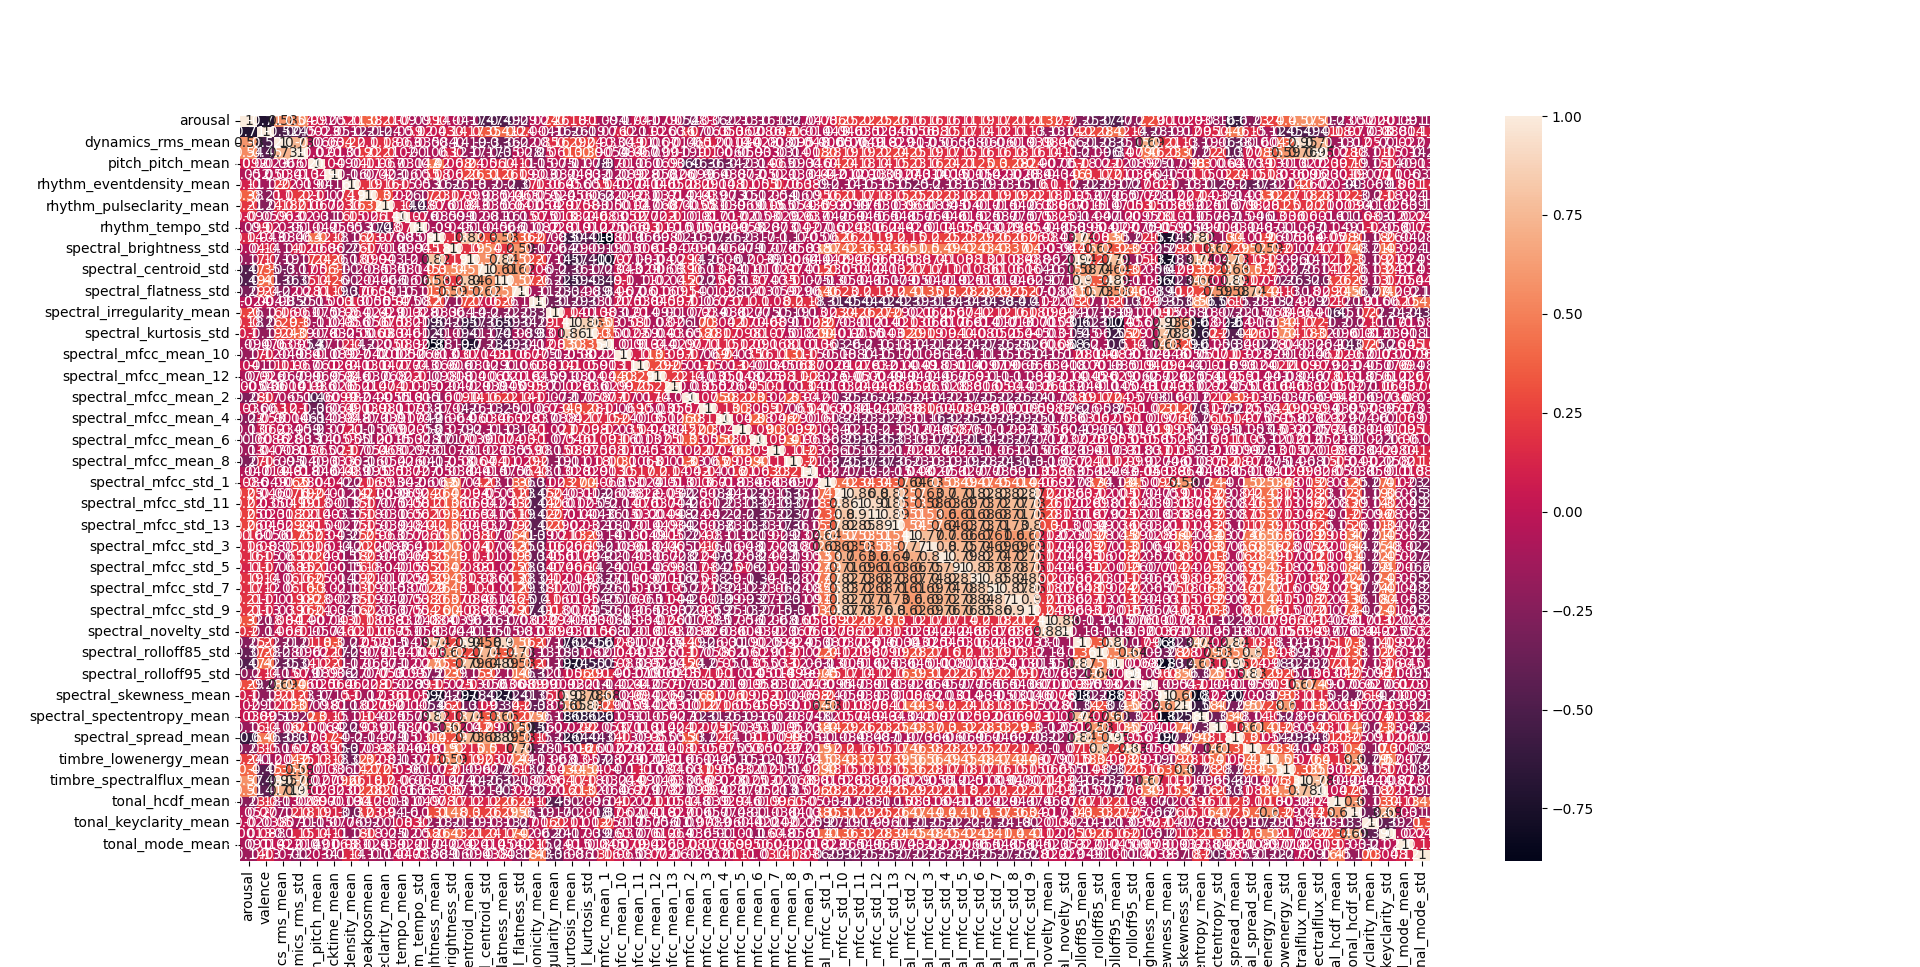
\includegraphics[width=0.4\textwidth]{Figures/Figure_1.png}
\end{figure}

\begin{figure}[h]
\caption{IADS-E Heatmap}
\centering
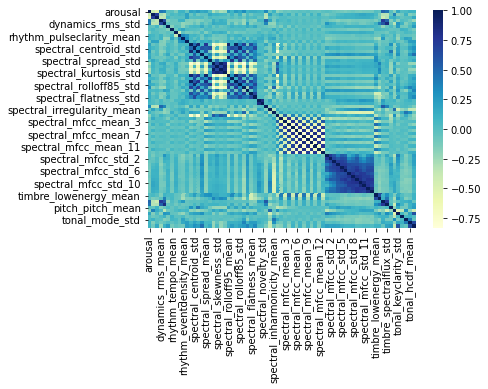
\includegraphics[width=0.4\textwidth]{Figures/iadheatmap.png}
\end{figure}

\FloatBarrier


\noindent
Using the Seaborn package, we can create a heatmap. This heatmap allows us to have a matrix representation of the values, where the colors represent the number of that value in the categories.

\begin{figure}[h]
\caption{EmoSoundscape Pairplot}
\centering
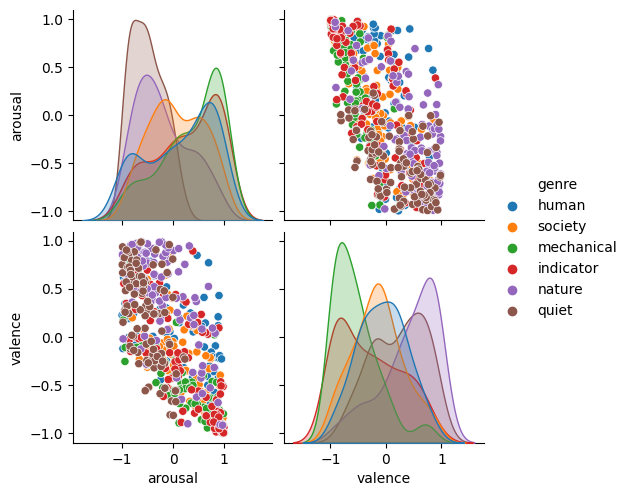
\includegraphics[width=0.4\textwidth]{Figures/Figure_2.png}
\end{figure}

\begin{figure}[h]
\caption{IADS-E Pairplot}
\centering
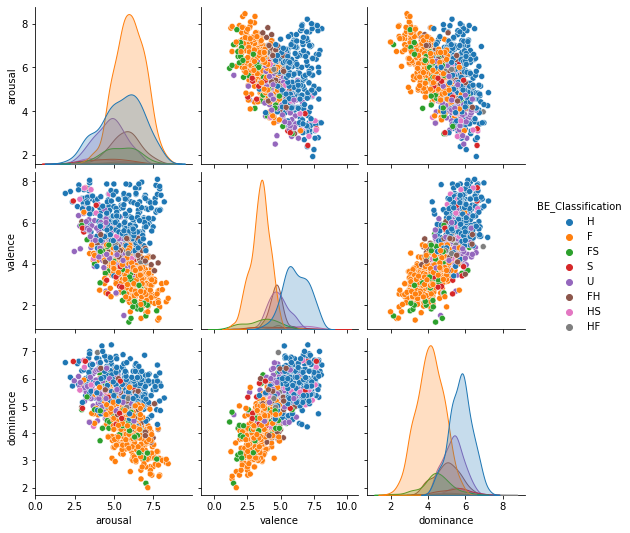
\includegraphics[width=0.4\textwidth]{Figures/iadpair.png}
\end{figure}

\FloatBarrier

\noindent
Using the Seaborn package again, we can create a pairplot. This pairplot allows us to see all the relationships between any two categories. In Figure 3, the pairplot shows the relationship between Arousal and Valence. It'll take too long to make a pairplot with all 70 numerical category columns. Figure 4 shows a pairplot between Arousal, Valence, and Dominance with BE Classification as Hue. Figure 5 shows us the correlation between Arousal and Dynamics. \\


\begin{figure}[h]
\caption{IADS-E Correlation between Arousal and Dynamics}
\centering
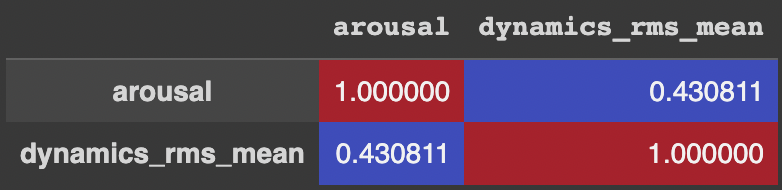
\includegraphics[width=0.4\textwidth]{Figures/iadsecorr.png}
\end{figure}

%-----------------------------------------------------------------------------------------------
\section{Preprocessing}
\label{sec:pre}

\noindent
Before we did any normalizing and standardizing, we checked to see if the datasets contained any missing values. Our method of checking this is using the function \emph{isnull().sum()}. Using this, EmoSoundscape yielded no missing values and IADS-E yielded 28 missing values. \\


\begin{figure}[h]
\caption{EmoSoundscape Min-Max Scaling}
\centering
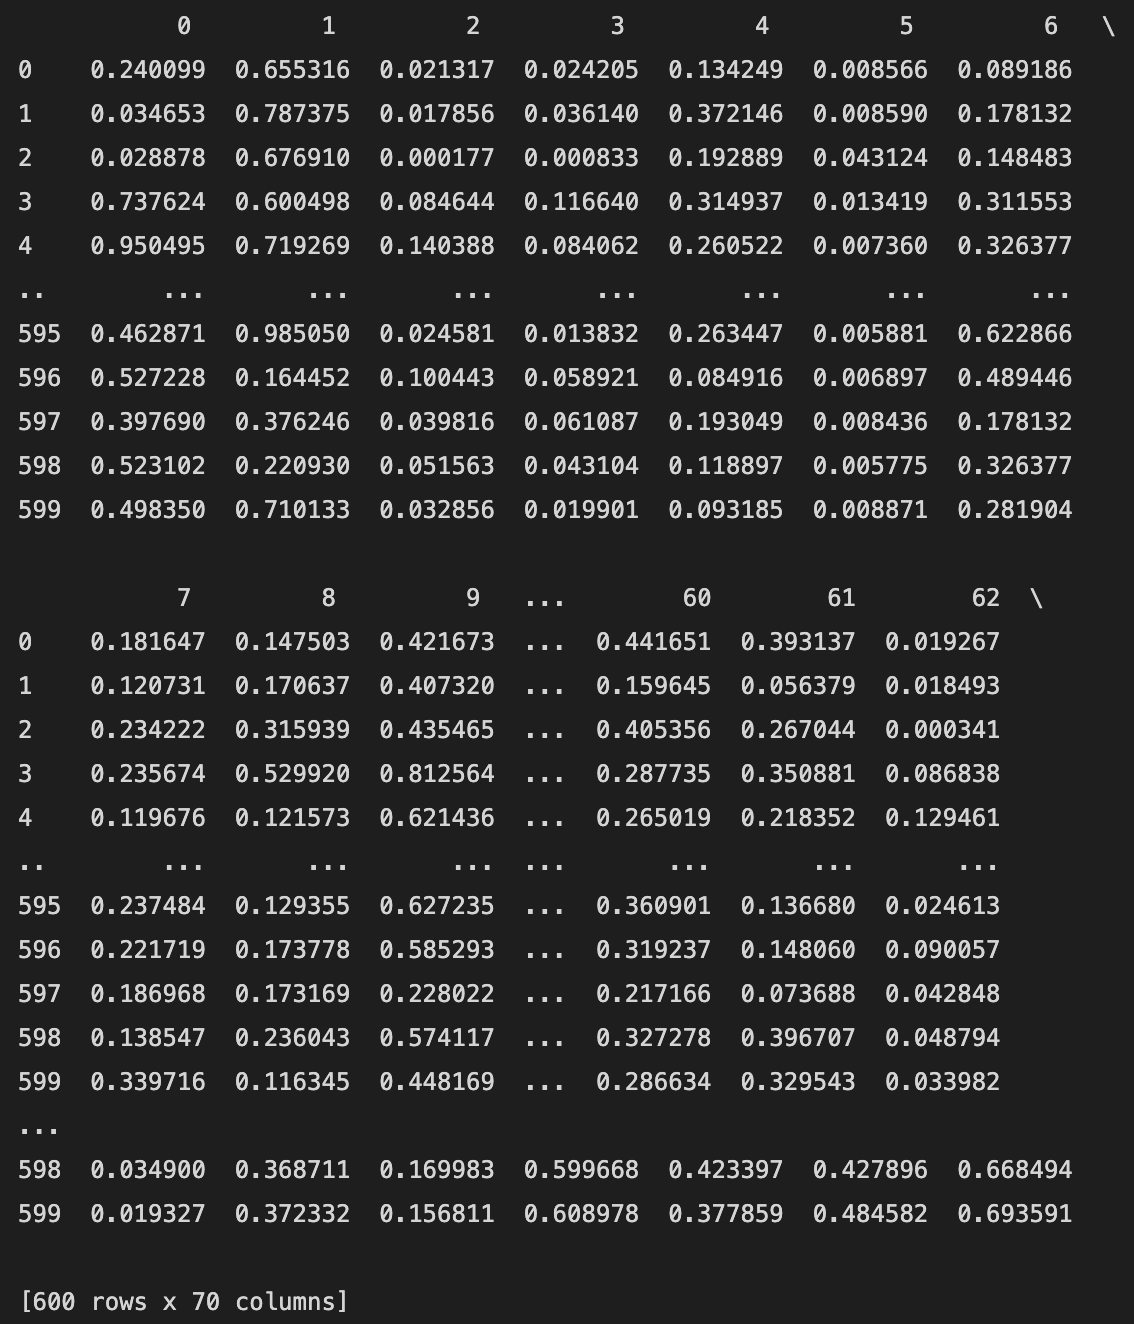
\includegraphics[width=0.40\textwidth]{Figures/min_max_1.png}
\end{figure}

\FloatBarrier

\begin{figure}[h]
\caption{IADS-E Min-Max Scaling}
\centering
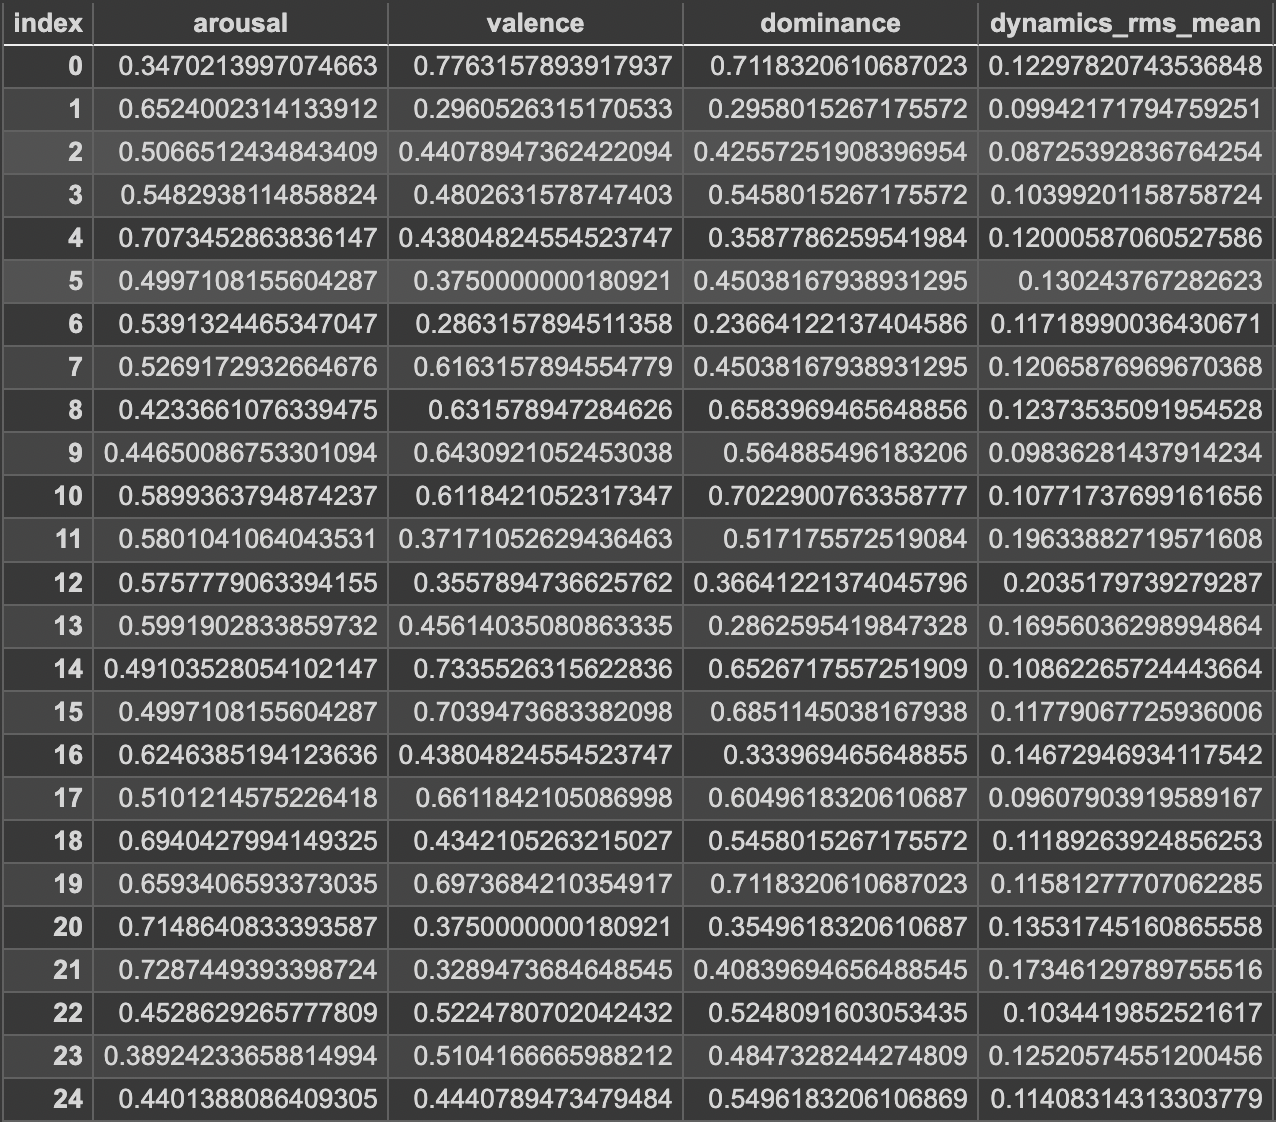
\includegraphics[width=0.40\textwidth]{Figures/IADSEScaledDf.png}
\end{figure}


\noindent
All the numerical category columns were normalized using min-max scaling. This is so that we can convert all values of different scopes and origins to a common scale. The python library used is Sklearn, which allowed us to do min-max scaling. \\

\FloatBarrier


\begin{figure}[h]
\caption{EmoSoundscape One-Hot Encoding}
\centering
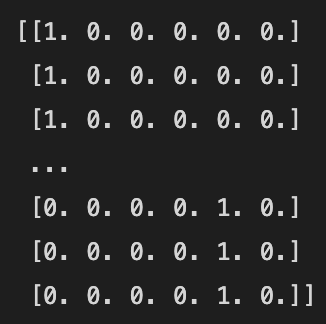
\includegraphics[width=0.25\textwidth]{Figures/one_hot_1.png}
\end{figure}

\FloatBarrier


\noindent
In the EmoScoundscape dataset, the first 5 columns were categorical columns. The column that made the most sense to preprocess is the genre column. We applied one-hot encoding using the same python library, Sklearn, to this column to represent the categorical values as binary vectors. \\


\noindent
Before applying linear and non-linear regression to the model, we split the preprocessed datasets. EmoSoundscape was split into an 60:20:20 ratio, and the columns used for prediction and evaluation were valence and arousal. In the case of the IADS-E dataset, the data was split into 80:20 and all the columns were used as features and the target was dominance.\\

%-------------------------------------------------------
\section{Prediction Models}
\label{sec:models}

\noindent
Linear and non-linear regression were applied to both EmoSoundscape and IADS-E. The data were plotted and the train, evaluation, and test RMSE were recorded. For IADS-E, we used Linear Regression and Support Vector Regression to predict Dominance.\\

\begin{figure}[h]
\caption{EmoSoundscape Dataset with Linear Regression}
\centering
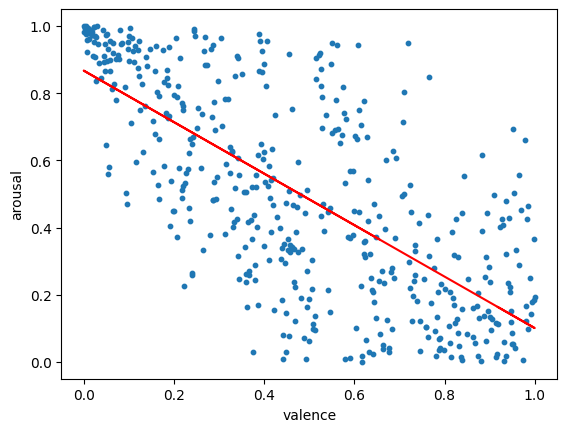
\includegraphics[width=0.5\textwidth]{Figures/emosound_lin.png}
\end{figure}

\begin{table}[h]
\caption{EmoSoundscape Linear Regression RSME}
\begin{center}
\begin{tabular}{ |c|c| } 
 \hline
 Training RMSE & 0.20959917010509416 \\ 
 Evaluation RMSE & 0.21643420242168082 \\ 
 Testing RMSE & 0.24782303310822504 \\ 
 \hline
\end{tabular}
\end{center}
\label{tab:myTab}
\end{table}

\FloatBarrier

\begin{figure}[h]
\caption{EmoSoundscape Dataset with Non-Linear Regression}
\centering
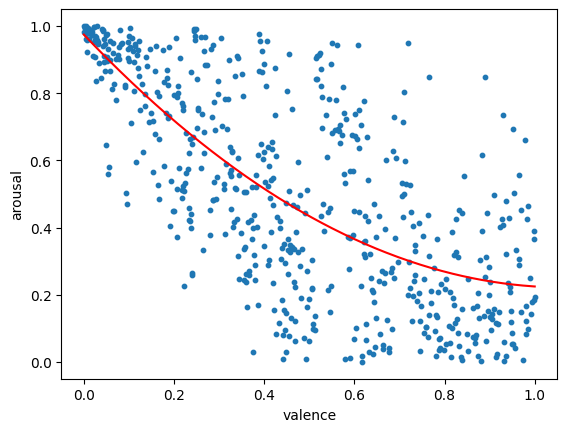
\includegraphics[width=0.5\textwidth]{Figures/emosound_nonlin.png}
\end{figure}

\begin{table}[h]
\caption{EmoSoundscape Non-Linear Regression RSME}
\begin{center}
\begin{tabular}{ |c|c| } 
 \hline
 Training RMSE & 0.3418957907106979 \\
 Evaluation RMSE & 0.5162349898576831 \\
 Testing RMSE & 0.21294143281833983 \\
 \hline
\end{tabular}
\end{center}
\label{tab:myTab}
\end{table}

\FloatBarrier


The EmoSoundscape dataset used valence and arousal to evaluate and predict the model. Linear regression displays a straight slope as its prediction, while non-linear regression has more of a concave curve, fitting the data a lot more. The RSME is not too far off from 0. The IADS-E dataset used all the columns as features to predict Dominance. The linear model used is Linear Regression and Support Vector Regression was used as the non-linear model. The accuracy was better for Support Vector Regression.\\

5-fold cross-validation was applied to both the linear and non-linear models to better tune them. 
\FloatBarrier

\begin{figure}[h]
\caption{IADS-E Dataset with Linear Regression}
\centering
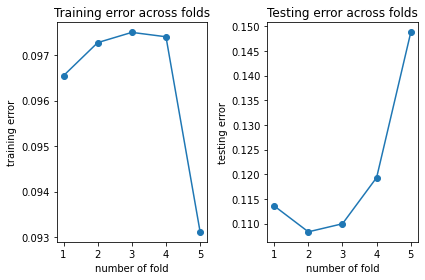
\includegraphics[width=0.4\textwidth]{Figures/5FoldLR.png}
\end{figure}

\FloatBarrier

\begin{figure}[h]
\caption{IADS-E Dataset with Linear Regression}
\centering
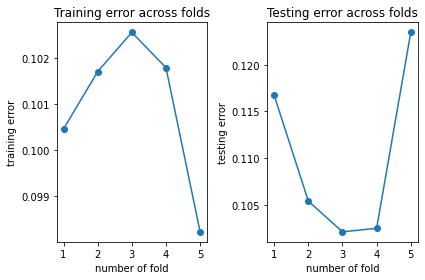
\includegraphics[width=0.4\textwidth]{Figures/5FoldErrorGraph.png}
\end{figure}

\begin{table}[h]
\caption{EmoSoundscape Linear with Cross Validation}
\begin{center}
\begin{tabular}{ |c|c| } 
 \hline
 Accuracy & 0.218 \\
 Standard Deviation of Accuracy & 0.468 \\
 Overall RMSE & 0.705 \\
 \hline
\end{tabular}
\end{center}
\label{tab:myTab}
\end{table}

\begin{table}[h]
\caption{EmoSoundscape Non-Linear with Cross Validation}
\begin{center}
\begin{tabular}{ |c|c| } 
 \hline
 Accuracy & 0.277 \\
 Standard Deviation of Accuracy & 0.378 \\
 Overall RMSE & 0.667 \\
 \hline
\end{tabular}
\end{center}
\label{tab:myTab}
\end{table}

\FloatBarrier

\begin{table}[h]
\caption{IADS-E Linear with Cross Validation}
\centering
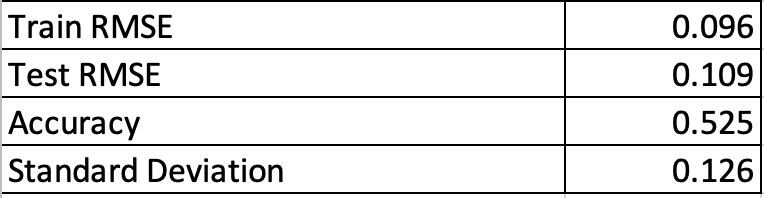
\includegraphics[width=0.3\textwidth]{Figures/LR_Data.png}
\end{table}

\FloatBarrier

\begin{table}[h]
\caption{IADS-E SVR with Cross Validation}
\centering
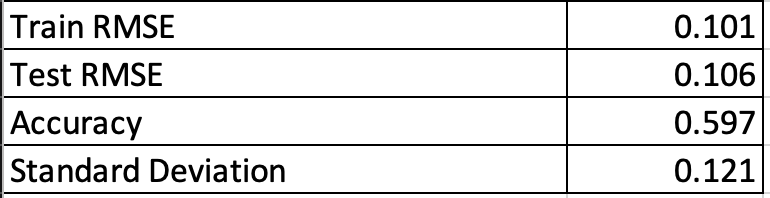
\includegraphics[width=0.3\textwidth]{Figures/SVR_Data.png}
\end{table}

\FloatBarrier


\noindent
We can see that when linear regression is applied to EmoSoundscape, the plot shows underfitting, as it doesn't accurately catch all the data. When non-linear regression is applied to Emosoundscape, it shows a fairly good fit of the data at degree 2. However, increasing the non-linear regression degree will cause the model to overfit. In the case of IADS-E, both the models show underfitting, however, Support Vector Regression is more accurate than Linear Regression. We can improve the models by preprocessing data like managing outliers, feature selection, and increasing the complexity of the model. We can also try other models to see which ones perform the best.\\
}

\noindent
We applied feature selection and dimensionality reduction techniques to get better test errors and to tackle the Curse of Dimensionality. Linear Principal Component Analysis (PCA) from dimensionality reduction and f\_regression from feature selection was applied on top of the EmoSoundscape dataset. Linear PCA is a method to find a linear mapping to project the data into low-dimensional space via principal components such that the variances of the low-dimensional representation are maximized. The libraries used to accomplish this is PCA from sklearn.decomposition and it was run with 2 features. F\_regression is a method to determine correlation between features. The libraries used to accomplish this are SelectKBest and f\_regression from sklearn.feature\_selection and it was run with 70 features (all the numerical data and the categorical data were dropped).\\

\begin{figure}[h]
\caption{EmoSoundscape with Linear PCA}
\centering
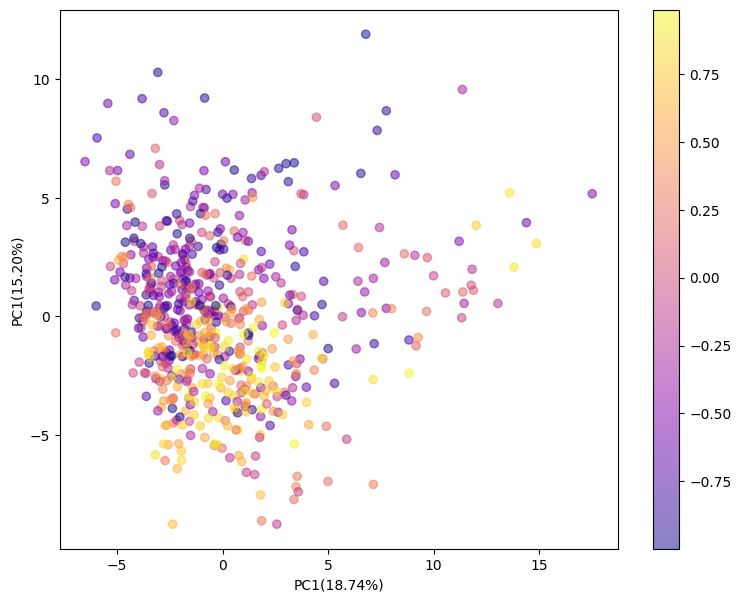
\includegraphics[width=0.4\textwidth]{Figures/emosound_pca.png}
\end{figure}

\FloatBarrier

\noindent
Figure 13 displays the plotted dataset, where the colored bar on the side represents the eigenvalue--that shows how much original variance is covered. So whatever color the data point is corresponds to that eigenvalue. \\

\begin{figure}[h]
\caption{EmoSoundscape with F\_Regression}
\centering
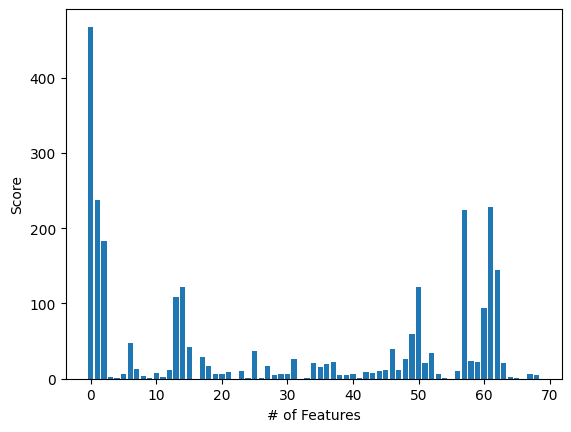
\includegraphics[width=0.3\textwidth]{Figures/emosound_f_reg.png}
\end{figure}

\FloatBarrier

\noindent
Figure 14 displays a bar graph, where the y axis represents the score. The higher the score, the more "important" it is when n number of features is used. \\

\begin{table}[h]
\caption{EmoSoundscape Test RMSE Using New Methods}
\begin{center}
\begin{tabular}{ |c|c| } 
 \hline
 Linear PCA & 8.547263602864924e-15 \\
 f\_regression & 0.3530360375440061 \\
 \hline
\end{tabular}

\end{center}
\label{tab:myTab}
\end{table}
\FloatBarrier

\noindent
For the IADSE dataset, we used the f-regression and Backward Elimination to reduce the number of features from 76 to 10. Using the f-regression, we filter out all the columns and select the best 10 features. Similarly, Using a technique called 'Backward Elimination' we reduce the number of features to 10. \\

\begin{table}[h]
\caption{IADS-E Linear Test RMSE after Feature Selection}
\begin{center}
\begin{tabular}{ |c|c| } 
 \hline
 selectKBest(f-regression) & 0.108 \\
 Backward Elimination & 0.102 \\
 \hline
\end{tabular}

\end{center}
\label{tab:myTab}
\end{table}

\begin{table}[h]
\caption{IADS-E SVR Test RMSE after Feature Selection}
\begin{center}
\begin{tabular}{ |c|c| } 
 \hline
 selectKBest(f-regression) & 0.105 \\
 Backward Elimination & 0.101 \\
 \hline
\end{tabular}

\end{center}
\label{tab:myTab}
\end{table}
\FloatBarrier
\begin{figure}[h]
\caption{IADSE Evaluation Metrics}
\centering
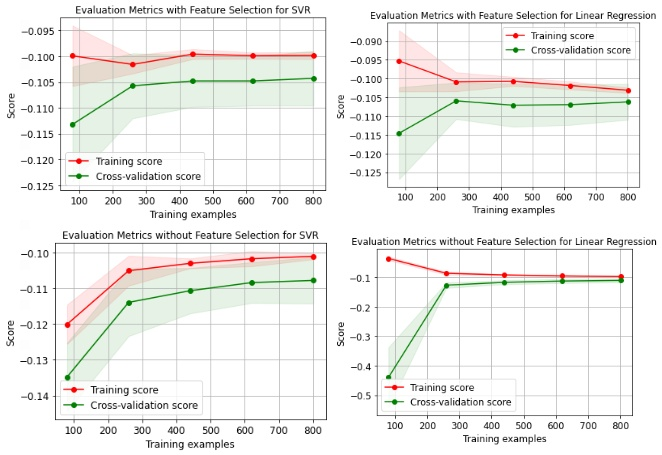
\includegraphics[width=0.5\textwidth]{Figures/combine_images.jpeg}
\end{figure}

\FloatBarrier

\noindent
Backward elimination fits a linear model on the independent variables and finds out their p-value. We pass a parameter 'n\_features\_to\_select' to select the number of features and a 'direction' to choose between forward selection and backward elimination. It reduces the number of features by eliminating the feature that has the highest p-value. It repeats the process till 10 features are left. We selected different 'number of features' and found that selecting 10 features gave us the highest accuracy. The python library used for this is scikit Learn's feature\_selection. We import the SequentialFeatureSelector to run Backward Elimination and selectKBest and f-regression for f-regression.\\
%-------------------------------------------------------
\section{Computational Resources}
\label{sec:models}

\noindent
The EmoSoundcsape model was made on a Windows 11 desktop PC. The specification of the PC has an Intel i7-12700k, 32GB of ram, and an NVIDIA RTX 3080. The IADS-E dataset was modeled on an M1 pro MacBook pro with an integrated GPU and 16 GB RAM. All the Python libraries are using the latest Python version: 3.10.5.\\

%-------------------------------------------------------
\section{Comparison and Analysis}
\label{sec:models}
\noindent
We can see some differences between the test RMSE between the model with feature selection/dimensionality reduction and the model without it. The EmoSoundscape model with linear regression had a test RMSE of 0.24782303310822504 and with non-linear regression, the test RMSE was 0.21294143281833983. Now, applying linear PCA, the test RMSE yielded 8.547263602864924e-15. The error was suspiciously low, and it may be because the dataset was modified differently with preprocessing.StandardScaler() and PCA. When applying f\_regression to the Emosoundscape, the test RMSE is slightly higher, at 0.3530360375440061. For the IADS-E dataset, the RMSE difference between the original models and the FS/DR models was significant using Backward Elimination and very little for f-regression. Without feature selection, the test RMSE for the Linear Model was 0.109 and for SVR it was 0.106. After f-regression FS/DR, both the values dropped to 0.108 and 0.105 respectively and for Backward Elimination, it was 0.102 and 0.101 respectively. Even though the test RMSE difference is low, the accuracy improved by 8\% and 5\% for Linear and SVR respectively.\\

\noindent
The Emosoundscape dataset preparation was different when each technique is applied, the one similarity is that the first 5 categorical data columns is dropped. When applying linear and non-linear regression, the dataset is split into data X and target Y, where X is the valence column and Y is the arousal column. That dataset already is Min-Max scaled. With linear PCA, the whole dataset is fed into the model, where it was scaled and transformed. The difference with this one is that Min-Max wasn't used. With f\_regression, X is changed so it now includes all the columns, except the first 5 categorical data columns. Since f\_regression looks at features, I wanted to incorporate all the columns to see if the results yields a better RMSE. In the case of IADS-E dataset, all the features were used initially to train the model except for the categorical features and they were scaled using the min-max scaler. Then after feature selection, we got it down to 10 features for maximum accuracy.

%-------------------------------------------------------
\section{Conclusion}
\label{sec:models}
\noindent
The intentions were to analyze the EmoSoundscape and IADSE-E and create models to determine the RMSE and accuracy, which we were able to do successfully. More effort could've been put towards preprocessing because it seems like applying feature selection and dimensionality reduction doesn't give a big enough jump improvement when compared to linear and non-linear regression. We thought of methods like hyper-parameter tuning should be considered as a potential technique to use.

%-------------------------------------------------------
\bibliographystyle{IEEEtran}
\bibliography{IEEEfull,sample-base}

\end{document}
